\documentclass{article} %\documentclass[final,10pt,reqno, oneside, dvipsnames]{article}

\usepackage[utf8]{inputenc}
\usepackage[a4paper, total={8in,10in}, includeheadfoot]{geometry}

\usepackage{graphicx}
\usepackage{placeins}
\usepackage{tabularx}

%\setlength{\textwidth }{8.00 in}
%\setlength{\textheight}{9.25 in} % \textheight     = 9.25 in
%\setlength{\oddsidemargin }{0.0 in}
%\setlength{\evensidemargin}{0.0 in}
%\setlength{\hoffset}{0.00 in}
%\setlength{\voffset}{-0.50 in}
%\setlength{\headsep}{12 pt}
%\setlength{\headheight}{14 pt}
%\setlength{\topmargin }{00 pt}
%\setlength{\topskip}{12 pt}
%\setlength{\footskip}{30 pt}
%\setlength{\parskip}{12 pt} % default: \parskip        = 12  pt
%\setlength{\parindent}{00 pt}

\usepackage{amsthm}
\usepackage{amsmath}
\usepackage{amssymb}
\usepackage{amsfonts}
\usepackage{graphicx}

\usepackage{fancyhdr}
\pagestyle{fancy}

\fancyhead{}
\fancyhead[LO]{\textbf{Wanzhu Zheng}}
\fancyhead[LE]{\textbf{Wanzhu Zheng}}
\fancyhead[CO]{\textbf{2024 WQ Final Programming Project Report}}
\fancyhead[CE]{\textbf{2024 WQ Final Programming Project Report}}
\fancyhead[RO]{\textbf{918166670}}
\fancyhead[RE]{\textbf{918166670}}

\usepackage{xcolor}
\newcommand{\rd}[1]{{\textcolor{red}{#1}}}

%%%%%%%%%%%%%%%%%%%%%%%%%%%%%%%%%%%%%% LOAD AMS LaTeX Packages %%%%%%%%%%%%%%%%%%%%%%%%%%%%%%%%%%%%%

\usepackage{listings}

% Format MATLAB code with the listings package
% Create a language setting for LaTeX
% One can change the language for each code-block optionally
% \lstset
% {
%     language=[LaTeX]TeX,
%     breaklines=true,
%     basicstyle=\tt\scriptsize,
%     keywordstyle=\color{blue},
%     identifierstyle=\color{magenta},
% }


% I like space between paragraphs, since it makes the document more readable. However, this does not
% seem to change the spacing between paragraphs contained in an item of a list.

\setlength{\parskip}{03pt} % default: \parskip = 12  pt

\usepackage{color}   % May be necessary if you want to color links

%%%%%%%%%%%%%%%%%%%%%%%%%%%%%%%%%%%%% EGP's LOCAL LaTeX MACROS %%%%%%%%%%%%%%%%%%%%%%%%%%%%%%%%%%%%%

\newcommand{\bs}[1]{\boldsymbol{#1}}


% The basic usage with the standard settings is straightforward. Just load the package in
% the preamble, at the end of all the other packages but prior to other settings.

% From the `Introduction' to the hyperref manual: Make sure it comes last of your loaded
% packages, to give it a fighting chance of not being over-written, since its job is to
% redefine many LATEX commands. Hopefully you will find that all cross-references work
% correctly as hypertext. For example, \section commands will produce a bookmark and a
% link, whereas \section* commands will only show links when paired with a corresponding
% \addcontentsline command.

%%%%%%%%%%%%%%%%%%%%%%%%%%%%%%%%%%%%%% TITLE, AUTHOR AND DATE %%%%%%%%%%%%%%%%%%%%%%%%%%%%%%%%%%%%%%

\title{2024 WQ Final Programming Project Report}
\author{Wanzhu Zheng} %YOUR NAME
\date{\today}
%\date{January 2022}

\begin{document}

\maketitle
\tableofcontents
\newpage

  \section{Problem Description}
    \label{SECT:SECTION 1}
    In today's digitalized world, image and pattern recognition play a vital role. This significance stems from their ability to automate mundane tasks that, although manageable by humans, can be viewed as inefficient uses of their time, such as digit or facial recognition. The objective of this project is to compare the effectiveness and accuracy of two algorithms: a basic algorithm and an SVD (Singular Value Decomposition) basis algorithm. Specifically, we aim to automate the identification of handwritten digits using data from the United States Postal Service (USPS). Automating this task is important because while humans are capable of recognizing digits, it is a mundane task that becomes prone to errors over time. In contrast, computers can perform this task much faster and with predetermined accuracy. By finding an image recognition algorithm that performs well, we can accomplish more in less time. This report explores the effectiveness of these two algorithms in achieving this objective, and we later conclude that SVD performs significantly better than our simple classification algorithm.

  \section{Data Set}
    \label{SECT:SECTION 2}
    We have access to a database named "USPS.mat" comprising handwritten digit data. This database consists of two main sets:
    \begin{itemize}
        \item training\_set
        \item test\_set
    \end{itemize}
    Each set contains patterns of digits along with their corresponding labels. 
    \noindent The training set consists of two components: 
    \begin{enumerate}
        \item \emph{Train patterns}: These are patterns of handwritten digits stored in a matrix of size $256 \times 4649$. Each digit pattern is represented by a raster scan of $16 \times 16$ gray level pixel intensities normalized to $[-1,1]$.
        \item \emph{Train labels}: This matrix is of size $10 \times 4649$ and contains the classification labels for the digits in the training set. It provides the true information about the digit images.
    \end{enumerate}
    Similarly, the test set also comprises of two components:
    \begin{enumerate}
        \item \emph{Test patterns}: Like the training set, this matrix is of size $256 \times 4649$ and contains patterns of handwritten digits. Each digit pattern is represented by a raster scan of $16 \times 16$ gray level pixel intensities normalized to $[-1,1]$.
        \item \emph{Test labels}: This matrix, sized $10 \times 4649$, contains the classification labels for the digits in the test set, providing the true information about the digit images. error is minimized.
    \end{enumerate}

    \noindent The distinction between training and test data lies in the fact that training data contains known, expected outputs, typically gathered meticulously and validated by humans. Conversely, test data is the dataset upon which we aim to apply our model post-training phase. Normally, we lack knowledge of the correct outputs for test data, but in our case, this information is stored in the test labels. However, upon inspecting the test patterns, we observe that these digits are notably more chaotic compared to those in the training patterns. Consequently, we intend to evaluate our two distinct algorithms on these "noisy" digits subsequent to training them on the "clean" digits. This scenario exemplifies machine learning, where we initially train our model or algorithm on well-organized, pristine data before subjecting them to more disorderly data. You can find this dataset on public datasets such as Kaggle and OpenML. Provided below are the initial 16 images from our training dataset:
    \begin{figure}
        \centering
        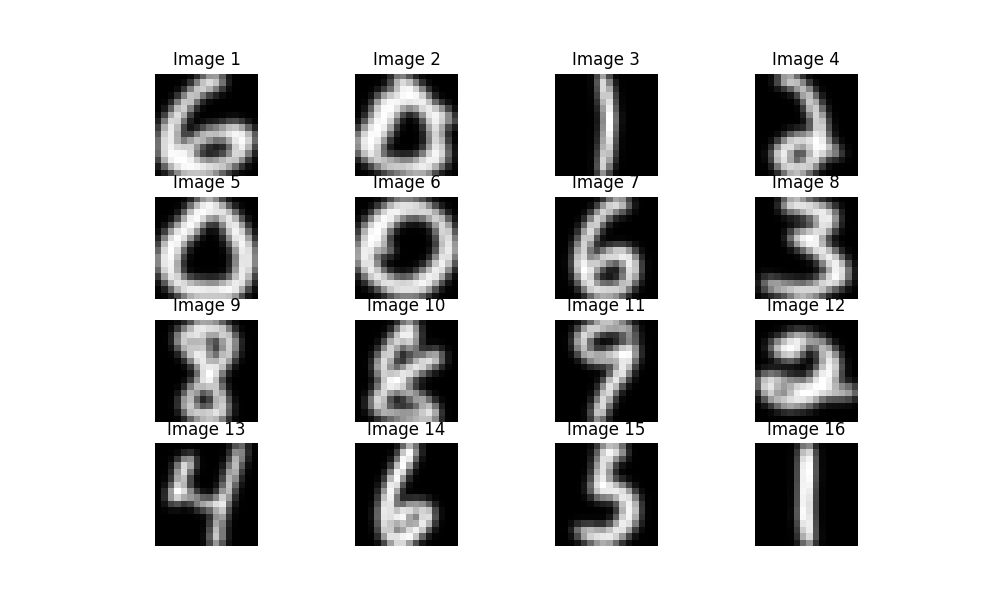
\includegraphics[width=9cm]{Figure_1.png}
        \caption{First 16 images in train\_patterns}
        \label{fig:fig1}
    \end{figure}

    \FloatBarrier

    \section{The Centroid Classification Algorithm}
        The centroid classification algorithm, also known as the nearest centroid classifier, is a simple yet effective method for classifying data points into predefined categories. It operates by calculating the centroid, or mean vector, for each class in the training dataset. During classification, the algorithm assigns a new data point to the class whose centroid is closest to it in terms of some distance metric, often Euclidean distance. In other words, the algorithm determines the class whose centroid is most similar to the input data point. The centroid classification algorithm is computationally efficient and straightforward to implement, making it particularly useful for tasks with relatively small datasets and low-dimensional feature spaces. However, it may not perform optimally in cases where classes are not well-separated or when the data distribution is highly irregular.
      \subsection{Description of the Algorithm}
        \label{SECT:SUBSECTION 3.1}
            The centroid classification algorithm computes the mean digits using our training data. This involves aggregating the pixel intensities corresponding to each digit (0 to 9) from our training patterns matrix and calculating the mean intensity for each pixel across all instances of that digit. For each digit, we determine the average pixel intensity for every pixel position based on the images in our training dataset. This process enables us to identify the typical gray level pixel intensities associated with each digit from our accurately labeled training data. We then replicate this procedure for the remaining digits, yielding the outcomes presented below:
            \begin{figure}[h]
                \centering
                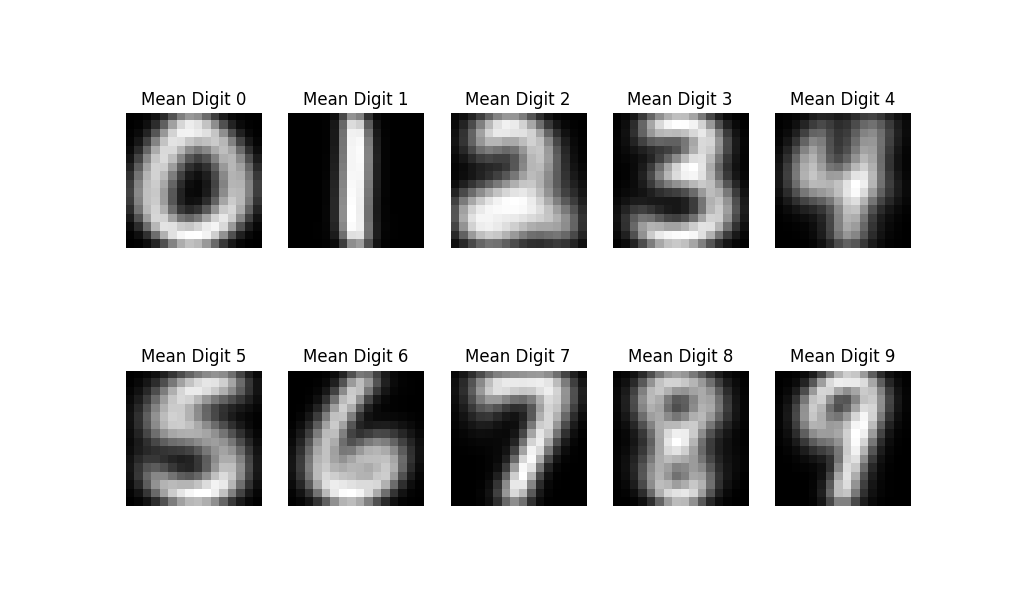
\includegraphics[width=9cm]{Figure_2.png}
                \caption{Images for Mean Digits}
                \label{fig:fig2}
            \end{figure}

            \FloatBarrier

          \subsection{Description of the Results}
            \label{SECT:SUBSECTION 3.2}
                A confusion matrix is a tabular representation that visualizes the performance of a classification model by comparing the actual labels of the dataset with the predicted labels made by the model. It provides a comprehensive overview of the model's performance across different classes. The matrix typically consists of rows and columns, where each row represents the actual class labels, and each column represents the predicted class labels. The diagonal of a confusion matrix represents the instances that are correctly classified by the model. In other words, the diagonal cells correspond to the true positives and true negatives. The cells of the matrix contain counts or proportions, indicating the number of data points that fall into each combination of actual and predicted classes. In a binary classification scenario, a confusion matrix has two rows and two columns, representing two classes: "positive" and "negative." The four possible outcomes are:
                \begin{itemize}
                    \item True Positive (TP): Instances correctly classified as positive.
                    \item False Positive (FP): Instances incorrectly classified as positive.
                    \item True Negative (TN): Instances correctly classified as negative.
                    \item False Negative (FN): Instances incorrectly classified as negative.
                \end{itemize}
                Below is the two confusion matrix developed for each algorithm:
                \begin{figure}[h]
                    \centering
                    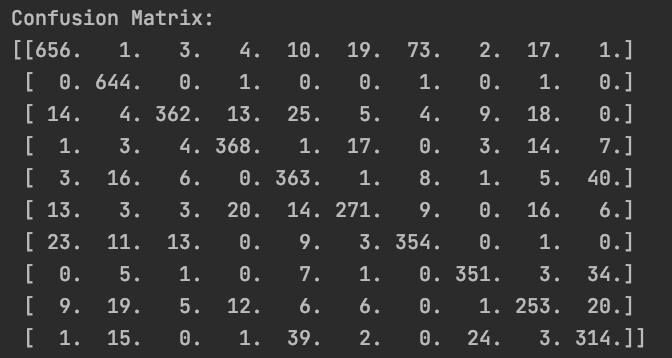
\includegraphics[width=9cm]{Conf_Matrix_1.png}
                    \caption{Confusion Matrix for Centroid Classification}
                    \label{fig:fig3}
                \end{figure}

            \FloatBarrier
            \noindent The diagonal elements represent the instances that are correctly classified. For example, the number 656 in the top-left corner indicates that 656 instances of the number $0$ were correctly classified as $0$, while the number 644 in the second row and second column indicates that 644 instances of the number $1$ was correctly classified as $1$. The off-diagonal elements represent mis-classifications. For example, the element in row 1, column 2 indicates that 1 instance of the number $0$ were misclassified as the number $1$. The numbers along each row provide information about the distribution of instances across different classes. For example, in the first row, there are a total of 786 instances of the number $0$. \\


  \section{The SVD Classification Algorithm}
    Singular Value Decomposition (SVD) is a fundamental matrix factorization technique in linear algebra. It is widely used across various fields, including signal processing, image compression, data analysis, and machine learning. Mathematically, given a matrix $A$ of size $m\times n$, SVD decomposes it into three constituent matrices:
    \begin{equation}
        A = U\Sigma V^T
    \end{equation}
    where:
    \begin{itemize}
        \item $U$ is an $m\times m$ orthogonal matrix representing the left singular vectors
        \item $\Sigma$ is an $m \times n$ diagonal matrix with non-negative real numbers on the diagonal, known as the singular values
        \item $V^T$ is an $n \times n$ orthogonal matrix representing the right singular vectors
    \end{itemize}
    The SVD classification algorithm is a machine learning method that leverages the SVD technique for pattern recognition and classification tasks. In this algorithm, the SVD is applied to decompose the training data matrix into three matrices: the left singular vectors (representing features), the singular values (indicating their importance), and the right singular vectors (representing classes or categories). These matrices capture essential information about the underlying structure of the data.
    \subsection{Description of the Algorithm}
        \label{SECT: SECTION 4.1}
            Our algorithm for SVD classification is specified as follows:
            \begin{enumerate}
                \item \textbf{Pooling Data Images:} Let $X_k$ represent the matrix of images corresponding to the $k^{th}$ digit train patterns. This matrix is obtained by pooling together all images for digit $k$
                \begin{equation*}
                    X_k = {x_1^k, x_2^k, \hdots, x_i^k}
                \end{equation*}
                where $x_i^k$represents the $i^{th}$ image corresponding to the $k^{th}$ digit
                \item \textbf{Computing Rank-17 SVD:} For matrix $X_k$ the rank-17 SVD is computed as:
                \begin{equation*}
                    X_k = U_k \Sigma_k V_k^T
                \end{equation*} where $U_k$ is an $m \times 17$ matrix containing the left singular vectors, $\Sigma_k$ is a $17 \times 17$ diagonal matrix containing the singular values, $V_k^T$ is a $17 \times n$ matrix containing the right singular vectors.
                In our report, only the first $17$ singular values and corresponding vectors are computed.
                \item \textbf{Storing Left Singular Vectors:} The left singular vectors of matrix $X_k$ are stored in an array of size $256 \times 17 \times 10$. 
                \item \textbf{Expansion Coefficients Calculation:} Now, for each test digit image $j$ and each digit class $k$, we want to compute the expansion coefficients with respect to the $17$ singular vectors obtained from the training digit image set. Again, let $U_k$ denote the matrix containing the left singular vectors for digit class where each column represents a singular vector and $X_j$ denote the test digit image matrix. To compute the expansion coefficients $c_{kj}$, we perform:
                \begin{equation*}
                    c_{kj} = U_k^T X_j
                \end{equation*}
                \item \textbf{Storage in 3D Array:} The resulting coefficients are stored in a 3-D array
            \end{enumerate}
        \subsection{Description of the Results}
            \label{SECT: SECTION 4.2}
            We can directly compute the approximation by taking the dot product of the left singular vectors $U_k$ for the $k^{th}$ digit class and the expansion coefficients found earlier. Once we have the rank 17 approximation for each test digit image, we compute the error between the original test digit image and its approximation. This error represents how well the approximation captures the features of the original image. The error can be computed using a suitable distance metric, such the 2-norm, between the original image and its approximation. The rationale behind computing the error is to determine which class the test digit image belongs to. The classification idea is that a test digit image should be assigned to the class of the $k^{th}$ digit if its corresponding rank 17 approximation has the smallest error among the approximations obtained using the left singular vectors from all classes. By computing the error for each test digit image with respect to each class, we can identify the class that provides the best approximation and assign the test digit image to that class. Below is the confusion matrix for SVD classification:
            \begin{figure}[h]
                \centering
                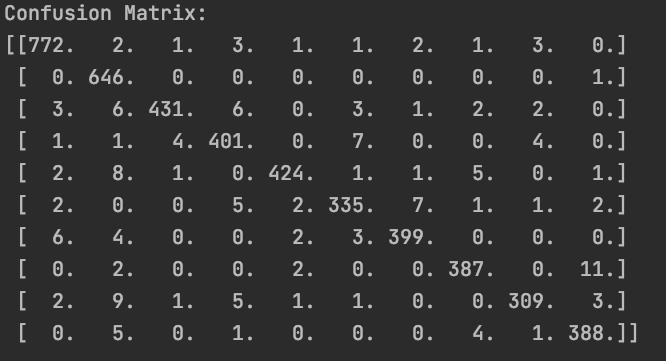
\includegraphics[width=9cm]{Conf_Matrix_2.png}
                \caption{Confusion Matrix for SVD Classification}
                \label{fig:fig4}
            \end{figure}

            \FloatBarrier
            
            \noindent The diagonal elements represent the instances that are correctly classified. For example, the number 772 in the top-left corner indicates that 772 instances of the number $0$ were correctly classified as $0$, while the number 646 in the second row and second column indicates that 646 instances of the number $1$ was correctly classified as $1$. The off-diagonal elements represent mis-classifications. For example, the element in row 1, column 2 indicates that 2 instances of the number $0$ were misclassified as the number $1$. The numbers along each row provide information about the distribution of instances across different classes. For example, in the first row, there are a total of 786 instances of the number $0$. \\
            
            \noindent By analyzing the distribution of correct and incorrect classifications across different classes, we can assess the overall performance of the classification model. High values along the diagonal and low values off the diagonal indicate good performance, while patterns of mis-classifications can highlight areas where the model may need improvement.
            
  \section{Analysis}
  Below, we provide two tables that summarize the accuracy of classifications for both algorithms based on their respective confusion matrices. We choose to analyze accuracies because it's the best indicator for performance given that the clock-time of both algorithms are not significantly different. Therefore, given that speed is not a differentiating factor, we look at accuracy.

  \begin{center}
    \begin{table}[h]
        \caption{Centroid Classification Accuracy Table for Digits}
        \begin{tabular}{|l|l|l|l|l|l|l|l|l|l|l|}
        \hline
        Digit    & 0      & 1      & 2      & 3      & 4      & 5      & 6      & 7      & 8      & 9      \\
        \hline
        Accuracy & 0.9111 & 0.8932 & 0.9118 & 0.8783 & 0.7658 & 0.8338 & 0.7884 & 0.8977 & 0.7644 & 0.7441 \\
        \hline
        \end{tabular}
    \end{table}
    \begin{table}[h]
        \caption{SVD Classification Accuracy Table for Digits}
        \begin{tabular}{|l|l|l|l|l|l|l|l|l|l|l|}
        \hline
        Digit    & 0      & 1      & 2      & 3      & 4      & 5      & 6      & 7      & 8      & 9      \\
        \hline
        Accuracy & 0.9797 & 0.9458 & 0.9840 & 0.9525 & 0.9815 & 0.9544 & 0.9732 & 0.9675 & 0.9656 & 0.9557 \\
        \hline
        \end{tabular}
    \end{table}
  \end{center}
  We observe that distinguishing the digit 9 poses the greatest difficulty, while identifying 2 is the most straightforward using the basic algorithm. This disparity may stem from the fact that the mean image for the digit 9 exhibits similarities with other digits, such as 7 or 8, to some extent. The basic algorithm's subpar performance can be attributed to its failure to account for variability within digit classes; for instance, variations in the formation of digit 1, such as the presence of a top tail, may lead to mis-classification as 7. Conversely, the ease of identifying digit 2 can be attributed to its distinctiveness from other digits. \\

  \noindent In contrast, with the SVD basis algorithm, we find that identifying 1 is the most challenging, while 2 remains the easiest. This discrepancy appears to be a consequence of how the SVD basis algorithm accommodates variations within digit classes, particularly evident in the diverse ways individuals write digit 1. For instance, the presence of a top tail in some instances of digit 1 may lead to mis-identification as 7. The challenge in distinguishing digit 1 contrasts with the straightforward identification of digit 2, which exhibits minimal variability across individuals' writing styles. \\

  \noindent Overall, from our two tables, we observe that SVD classification poses significantly higher accuracy compared to centroid classification. When considering their respective accuracies, the lowest accuracy achieved by the SVD basis algorithm is 94.58\%, surpassing the highest accuracy attained by our basic algorithm, which stands at 91.18\%. Therefore, even under its least favorable conditions, the SVD basis algorithm outperforms the basic algorithm, exhibiting a significant superiority. Notably, the SVD basis algorithm achieves a remarkable improvement of over 20\% accuracy compared to the basic algorithm, particularly evident in certain digits such as 4.

  \section{Conclusions}
  In our digital age, image and pattern recognition hold crucial importance for automating tasks that would otherwise consume human time, such as identifying digits or faces. This project aims to compare the efficiency and accuracy of two algorithms: a basic approach and an SVD basis algorithm. Our goal is to automate the identification of handwritten digits using USPS data. Automating this task is valuable because while humans can recognize digits, it's a mundane task prone to errors over time, whereas computers can perform it swiftly and accurately. \\
  
  \noindent This report assesses the effectiveness of these algorithms and concludes that the SVD approach outperforms the basic algorithm significantly in achieving our objective. We then introduce the "USPS.mat" database, containing handwritten digit data split into training and test sets. We aim to assess our algorithms' performance on these "noisy" digits after training them on the "clean" digits, highlighting the typical machine learning paradigm of training on organized data before handling more disorderly datasets. \\

  \noindent The centroid classification algorithm calculates the average digit images using the training data. It aggregates pixel intensities for each digit (0 to 9) from the training patterns matrix and computes the mean intensity for each pixel across all instances of that digit. This allows us to determine the typical gray level pixel intensities associated with each digit based on accurately labeled training data. The SVD classification algorithm involves decomposing the training data into its singular vectors. These singular vectors capture the essential features of the data. Then, for each test instance, the algorithm calculates expansion coefficients with respect to these singular vectors. By comparing these coefficients, the algorithm assigns the test instance to the class with the most similar representation, enabling classification. \\

  \noindent In our analysis, we find that the basic algorithm struggles most with distinguishing the digit 9, while identifying 2 is comparatively easier. Conversely, the SVD basis algorithm faces challenges in identifying digit 1 due to variations in its formation, yet excels in recognizing digit 2, which shows minimal variability. Overall, the SVD basis algorithm demonstrates significantly higher accuracy compared to the centroid classification. With accuracies ranging from 91.18\% to 94.58\%, the SVD basis algorithm outperforms the basic algorithm by over 20\% in certain cases. \\

  \noindent The report investigates the effectiveness of centroid and SVD basis algorithms in handwritten digit recognition, highlighting the latter's superiority in accuracy. Through meticulous analysis, the SVD basis algorithm consistently outperforms the centroid approach, particularly evident in challenging digit classifications, showcasing its potential for practical applications in image recognition tasks.

  \section{Computer Program}
    \begin{verbatim}
"""
Wanzhu Zheng
ID: 918166670
"""

from scipy import io
import matplotlib.pyplot as plt
import numpy as np

"""
Step 01: Download USPS.mat and plot the first 16 images
"""
data_dict = io.loadmat('USPS.mat')  # download USPS.mat
train_patterns = data_dict["train_patterns"]  # store train_patterns data
train_p2dArray = np.array(train_patterns)  # put train_patterns data into an array

fig = plt.figure(figsize=(10, 7))  # initialize a figure 10in wide, 7 in tall
rows = 4  # figure will have 4 rows
columns = 4  # and 4 columns

# get data for first 16 images
img1 = np.reshape(train_p2dArray[:, 0], (16, 16))
img2 = np.reshape(train_p2dArray[:, 1], (16, 16))
img3 = np.reshape(train_p2dArray[:, 2], (16, 16))
img4 = np.reshape(train_p2dArray[:, 3], (16, 16))
img5 = np.reshape(train_p2dArray[:, 4], (16, 16))
img6 = np.reshape(train_p2dArray[:, 5], (16, 16))
img7 = np.reshape(train_p2dArray[:, 6], (16, 16))
img8 = np.reshape(train_p2dArray[:, 7], (16, 16))
img9 = np.reshape(train_p2dArray[:, 8], (16, 16))
img10 = np.reshape(train_p2dArray[:, 9], (16, 16))
img11 = np.reshape(train_p2dArray[:, 10], (16, 16))
img12 = np.reshape(train_p2dArray[:, 11], (16, 16))
img13 = np.reshape(train_p2dArray[:, 12], (16, 16))
img14 = np.reshape(train_p2dArray[:, 13], (16, 16))
img15 = np.reshape(train_p2dArray[:, 14], (16, 16))
img16 = np.reshape(train_p2dArray[:, 15], (16, 16))

# for each img, create a subplot to the figure and plot the image in their corresponding subplot
fig.add_subplot(rows, columns, 1)
plt.imshow(img1, cmap='gray')
plt.axis('off')
plt.title("Image 1")

fig.add_subplot(rows, columns, 2)
plt.imshow(img2, cmap='gray')
plt.axis('off')
plt.title("Image 2")

fig.add_subplot(rows, columns, 3)
plt.imshow(img3, cmap='gray')
plt.axis('off')
plt.title("Image 3")

fig.add_subplot(rows, columns, 4)
plt.imshow(img4, cmap='gray')
plt.axis('off')
plt.title("Image 4")

fig.add_subplot(rows, columns, 5)
plt.imshow(img5, cmap='gray')
plt.axis('off')
plt.title("Image 5")

fig.add_subplot(rows, columns, 6)
plt.imshow(img6, cmap='gray')
plt.axis('off')
plt.title("Image 6")

fig.add_subplot(rows, columns, 7)
plt.imshow(img7, cmap='gray')
plt.axis('off')
plt.title("Image 7")

fig.add_subplot(rows, columns, 8)
plt.imshow(img8, cmap='gray')
plt.axis('off')
plt.title("Image 8")

fig.add_subplot(rows, columns, 9)
plt.imshow(img9, cmap='gray')
plt.axis('off')
plt.title("Image 9")

fig.add_subplot(rows, columns, 10)
plt.imshow(img10, cmap='gray')
plt.axis('off')
plt.title("Image 10")

fig.add_subplot(rows, columns, 11)
plt.imshow(img11, cmap='gray')
plt.axis('off')
plt.title("Image 11")

fig.add_subplot(rows, columns, 12)
plt.imshow(img12, cmap='gray')
plt.axis('off')
plt.title("Image 12")

fig.add_subplot(rows, columns, 13)
plt.imshow(img13, cmap='gray')
plt.axis('off')
plt.title("Image 13")

fig.add_subplot(rows, columns, 14)
plt.imshow(img14, cmap='gray')
plt.axis('off')
plt.title("Image 14")

fig.add_subplot(rows, columns, 15)
plt.imshow(img15, cmap='gray')
plt.axis('off')
plt.title("Image 15")

fig.add_subplot(rows, columns, 16)
plt.imshow(img16, cmap='gray')
plt.axis('off')
plt.title("Image 16")

plt.show()

"""
Step 02: Compute the mean digits in the train_patterns and put them in a matrix.
         Display the 10 mean digit images
"""
train_labels = data_dict["train_labels"]  # get train_labels data
train_aves = np.zeros((256, 10))  # initialize train_aves matrix
for k in range(10):
    digit_patterns = train_patterns[:, np.where(train_labels[k, :] == 1)[0]]  # select patterns for digit k
    mean_digit = np.mean(digit_patterns, axis=1)  # compute mean digit for k
    train_aves[:, k] = mean_digit  # store mean_digit into train_aves matrix
    plt.subplot(2, 5, k + 1)  # create subplots

    # plot the mean_digit image
    plt.imshow(np.reshape(mean_digit, (16, 16)), cmap='gray')
    plt.title('Mean Digit ' + str(k))
    plt.axis('off')

plt.show()

"""
Step 03: Conduct the simplest classification
"""
# (a)
test_patterns = data_dict["test_patterns"]  # store test_patterns data
test_classif = np.zeros((10, 4649))  # initialize test_classif matrix
for k in range(10):
    # compute squared Euclidean distances between test patterns and kth mean digit
    # distances = np.sum((test_patterns - np.tile(train_aves[:, k], (1, 4649))) ** 2)
    distances = np.sum((test_patterns - train_aves[:, k][:, np.newaxis]) ** 2, axis=0)
    test_classif[k, :] = distances  # store distances in test_classif matrix

# (b)
test_classif_res = [0] * len(test_classif[0])  # initialize test_classif_res list
# goal: find the position index of the minimum of each column of test_classif
for j in range(len(test_classif[0])):
    tmp = np.min(test_classif[:, j])
    ind = np.argmin(test_classif[:, j])
    test_classif_res[j] = ind  # return index in the jth position of matrix

# (c)
test_confusion = np.zeros((10, 10))  # initialize confusion matrix
test_labels = data_dict["test_labels"]  # store test_labels data
arr = np.array(test_classif_res)  # convert list to numpy array

# goal: gather the classification results for each digit
for k in range(10):
    tmp = arr[test_labels[k, :] == 1]  # get the classification results for the kth digit
    # count the occurrences of each result
    for j in range(10):
        test_confusion[k, j] = np.count_nonzero(tmp == j)

print("Confusion Matrix:")
print(test_confusion)  # print our confusion matrix

"""
Step 04: Conduct SVD-based classification computation
"""
# (a)
train_u = np.zeros((256, 17, 10))  # initialize matrix to 256x17x10
for k in range(10):
    tmp, tmp1, tmp2 = np.linalg.svd(train_patterns[:, train_labels[k, :] == 1])  # find SVD and store into 3 matrices
    train_u[:, :, k] = tmp[:, :17]  # store left singular vectors of the kth digit into the vector

# (b)
test_svd17 = np.zeros((17, 4649, 10))  # initialize matrix to 17x4649x10
for k in range(10):
    test_svd17[:, :, k] = train_u[:, :, k].T @ test_patterns  # compute 17 × 10 numbers for each test digit image
# print(test_patterns.shape) 256x4649


# (c)
# compute the error between each original test digit image
# and its rank 17 approximation using the kth digit images in the training dataset
test_svd17res = np.zeros((10, 4649))  # initialize matrix to 10x4649
for k in range(10):
    approx = train_u[:, :, k] @ test_svd17[:, :, k]  # find rank 17 approximation of test digits (256x4649)
    error = np.linalg.norm(test_patterns - approx, axis=0)  # calculate error between original test digit image and its rank 17 approximation
    test_svd17res[k, :] = error  # store error in matrix

# (d)
# compute the confusion matrix using the SVD-based classification method
test_svd17_confusion = np.zeros((10, 10))  # initialize the confusion matrix
test_classif_svd = np.argmin(test_svd17res, axis=0)  # find the position index of the minimum of each column

for kk in range(10):
    tmp_svd = test_classif_svd[test_labels[kk, :] == 1]  # get the classification results for the kkth digit
    for jj in range(10):
        test_svd17_confusion[kk, jj] = np.count_nonzero(tmp_svd == jj)  # count frequencies of "correct" and put them in confusion matrix

print("Confusion Matrix:")
print(test_svd17_confusion)  # print the confusion matrix

    \end{verbatim}

\end{document}
